In this section we discuss the future of time delay cosmography, and
present
% an ambitious yet realistic
a
roadmap of how this
measurement might be improved in the next decade. In order to construct the roadmap
(Section~\ref{ssec:roadmap}), we will discuss in detail how to
decrease the random uncertainties (increasing the precision of
the method,
Section~\ref{ssec:precision}), and the systematic uncertainties
that will
need to be controlled as the random uncertainties decrease
(thus maintaining high accuracy, Section~\ref{ssec:accuracy}).

However, before we lay out this roadmap, we first pause and
reflect on the broader context, and ask whether this is a worthy
endeavour.
% PJM: the following paragraph sounds similar to the introduction, I'm
% not sure it adds much.
%
% Understanding the nature of dark energy is one of the most
% profound questions in all of physics, and it is thus not surprising
% that the efforts of many scientists and funding agencies have been
% directed towards this goal. Dedicated instruments, telescopes, and
% satellites are being built or planned with budgets that range from the
% tens of millions of dollars into the billions (Euclid and
% WFIRST). Given the steep challenges associated with each technique,
% most scientist agree that is important to pursue several independent
% ones at the same time \citep{DETF,DESC}. First, we do not know which
% techniques will live up to their promise and which ones will be
% stymied by hitherto unknown systematic effects, when we reduce the
% random uncertainties by one or more orders of magnitudes. Second, as
% discussed in the introduction, extraordinary claims require
% extraordinay proof, so it will certainly require more than one
% independent measurement to convince the community that, for example,
% dark energy is not the cosmological constant ($w\neq-1$).
%
% Given this context, deciding whether time delay cosmography is worth
% pursuing boils down to three simpler questions.
%
This
boils down to three simpler questions. The first question is
whether time delays contain valuable information {\it independent} of
other cosmological probes. As detailed in Section~\ref{sec:cosmo}, the
answer is a resounding yes: gravitational time delays are virtually
independent of the uncertainties affecting the other established
probes of dark energy, and provide valuable complementary information,
chiefly on the Hubble constant, which is commonly regarded as one of
the essential ingredients for interpreting other datasets such as the
cosmic microwave background \citep{Hu05,Suy++12,Wei++13,Rie++16}.  We
will expand on this topic in the remainder of this section by showing
cosmological forecasts for gravitational time delays by themselves and
in combination with other probes.

The second question is whether it is feasible to achieve an {\it
interesting} level of precision and accuracy in coming years. In this
mindset, {\it interesting} is defined as having total uncertainties
comparable to that of other contemporary probes. This will be
discussed in detail in Sections~\ref{ssec:precision}
and~\ref{ssec:accuracy} below.

The third and final question is what is the {\it cost} of pursuing
this roadmap, and how this cost compares to that of other probes. Our aim is not
to compute a full cost accounting, which will be almost impossible
considering that each probe involves facilities, observatories,
computing and brainpower, well beyond the boundaries of any individual
project, collaboration, or funding agency (not to mention that the
marginal cost of adding a technique to an existing program or
facility is very different from what the cost of building a facility
just for that purpose; for example, the cost of monitoring strongly
lensed quasars in LSST data is much less than building and operating
the LSST). Instead, we will aim to give an approximate sense of the
observational and human resources that will be needed to pursue the
roadmap.

% PJM: the following sounded a bit more like a proposal, or an argued case, than
% a review, and maybe also a bit defensive?
%
% Having voted with our feet, we obviously think that the
% relatively low {\it cost} and the relatively low risk of time delay
% cosmology well justifies adding it to the investment portfolio of a
% modern cosmologist. Hopefully the rest of this section will give the
% reader enough information to make up their own mind on the matter.


% % % % % % % % % % % % % % % % % % % % % % % % % % % % % % % % % %

\subsection{Precision}
\label{ssec:precision}

With considerable observational and data analysis effort, the
feasibility of reaching a {\it precision} of 6-7\% in time delay distance
per lens has been demonstrated. The contributions to this statistical
error budget
from the time delay measurement, mass model, and environment
correction are at present approximately equal, and somewhat larger than
the estimated systematic errors. In this situation it makes sense to
enlarge the sample of lenses, in order to beat down the statistical
uncertainties. We return to the question of how to reduce the residual
systematic errors in the next section.

\citet{C+M09b} made initial Fisher matrix forecasts of the likely
available precision on $H_0$ in large future surveys. They considered
several possible samples, concluding that 100 well-measured systems
(with 5\% distance precision each) should provide sub-percent precision
on the Hubble constant, and provide  dark energy parameter constraints
that are competitive with optimistic forecasts of other ``Stage IV''
cosmological probes. They also note that comparable constraints could be
available from a sample of 4000 time delay lens systems, each with only
photometric redshifts and simple image configuration model constraints
\citep[following][]{Ogu07b,P+J10}.  Continued investigation of both samples
seems warranted, keeping in mind that the size of such a photometric
sample would be set by the availability of time delays measured at the
few percent level.

%%%%%%%%%%%%%%%%%%%%%%%%%%%%%%%%%
\begin{figure*}[!ht]
\centering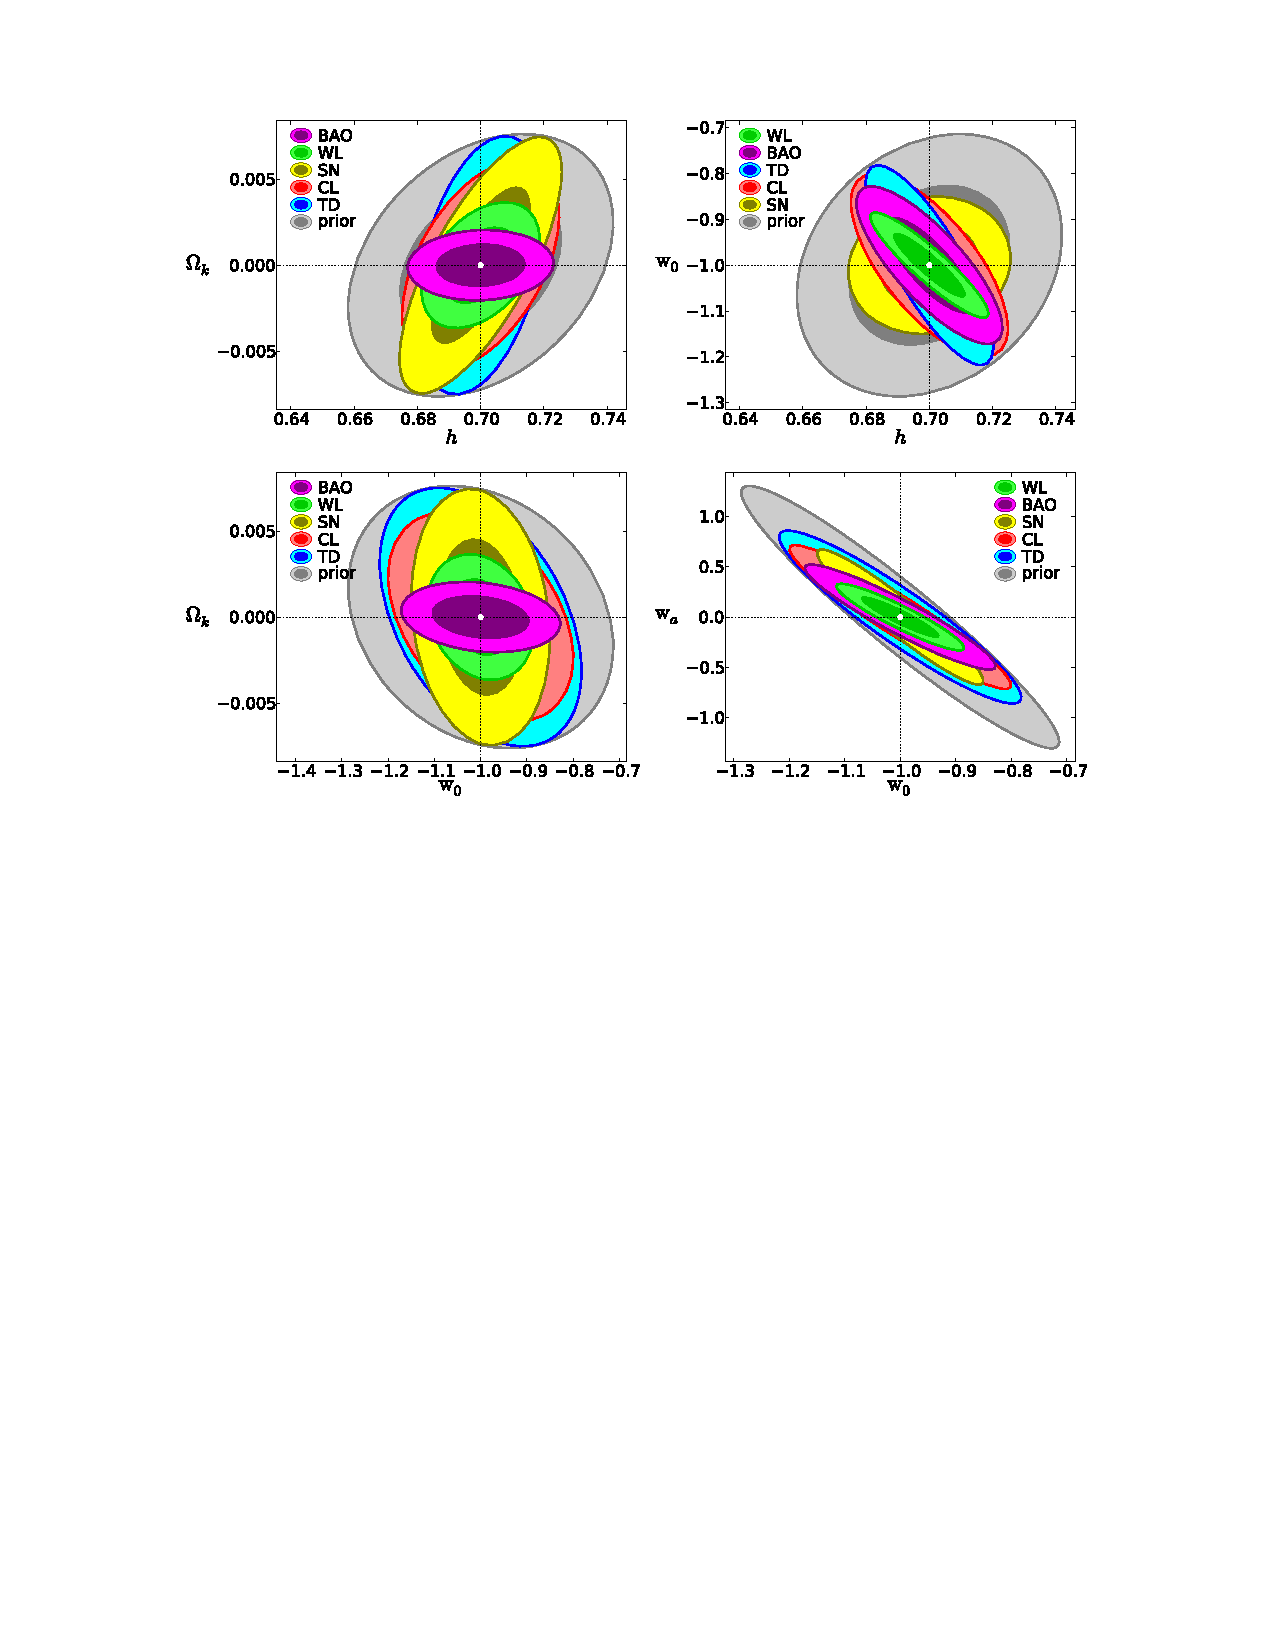
\includegraphics[width=0.9\linewidth]{figures/Coe+Moustakas09_fig14.pdf}
\caption{Fisher matrix forecasts of cosmological parameters, based on
Dark Energy Task Force assumptions and having 5\% distance precision
for each of 100 time delay lenses. The Stage IV cosmological probes
being compared in an  open CDM cosmological model with time-variable
dark energy equation of state are weak lensing (WL), BAO, supernovae
(SN), cluster mass function (CL) and time delay cosmography (TD).
Figure reproduced from \citet{C+M09b}.}
\label{fig:fisher}
\end{figure*}
%%%%%%%%%%%%%%%%%%%%%%%%%%%%%%%%%


While Figure~\ref{fig:fisher} allows different cosmological probes to
be compared (and assessed for competitiveness), it does not show the
value of combining those probes. Indeed, \citet{Lin11} found that the
particular combination of a type Ia supernova dataset with a time  delay
lens dataset holds promise, with a sample of 150 time delay distances,
each measured to 5\% precision, improving the dark energy figure of
merit by a factor of about 5 over what could be  plausibly obtained with
a sample of about 1000 Stage~III supernovae and a Planck CMB prior alone.

More recently, \citet{JeeKomatsuSuyu2015} have pointed out that
cosmological parameter forecasts for time delay lens samples are
conservative, if each lens is assumed only to measure the time delay
distance. Including the angular diameter distance dependence as well can
have a marked effect on the projection, especially if the spectroscopic
constraints on the lens mass distribution are assumed to be very strong.
The reproduction of Figure 5 from
\citet{JeeEtal2016} in the lefthand panel of Figure~\ref{fig:DdDdt}
illustrates this. These authors find that a future sample of
50 lenses
with 5\% measurements of both time delay distance and angular diameter
distance would increase the figure of merit by a factor of two over that
provided by a Stage~III supernova and BAO joint analysis. The righthand
panel of Figure~\ref{fig:DdDdt} puts such improvements in the  current
observational context. In the B1608$+$656 analysis, the  angular
diameter distance dependence {\it was} accounted for during the
calculation of the predicted time delay and velocity dispersion data,
but the constraints on the angular diameter distance were not strong:
assigning a uniform prior PDF for the cosmological parameters rather
than the distances introduced degeneracy between $\Dd$ and $\Ddt$,
which then seems to have been broken primarily by the time delay
information to yield a $5.7\%$ precision prediction for $\Ddt$, and
a corresponding $8.1\%$ precision prediction for $\Dd$.
With spatially resolved spectroscopy we should anticipate the angular
diameter distance becoming more important in future analyses, with
some work on simulated data needed to quantify this.


%%%%%%%%%%%%%%%%%%%%%%%%%%%%%%%%%
\begin{figure*}[!t]
\begin{minipage}{0.48\linewidth}
    \centering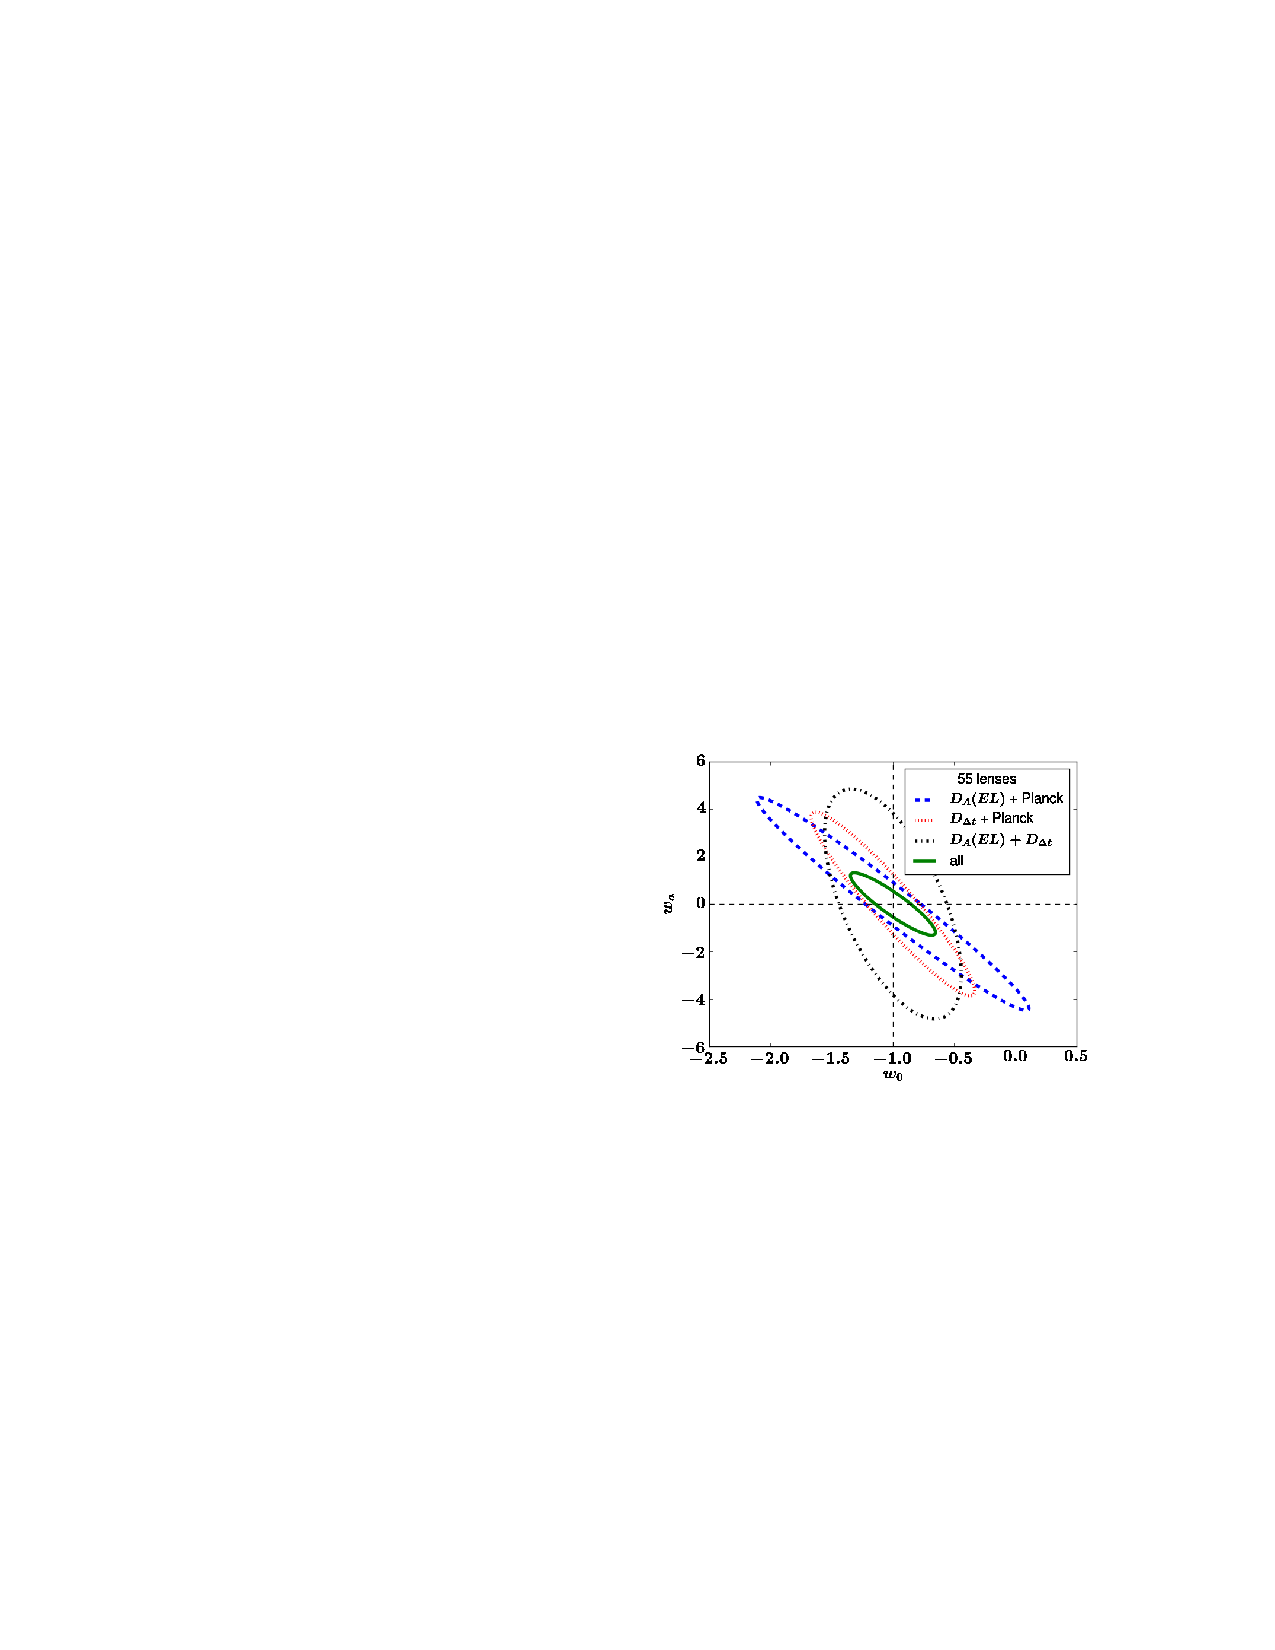
\includegraphics[width=\linewidth]{figures/Jee16_fig5b.pdf}
\end{minipage}\hfill
\begin{minipage}{0.48\linewidth}
    \centering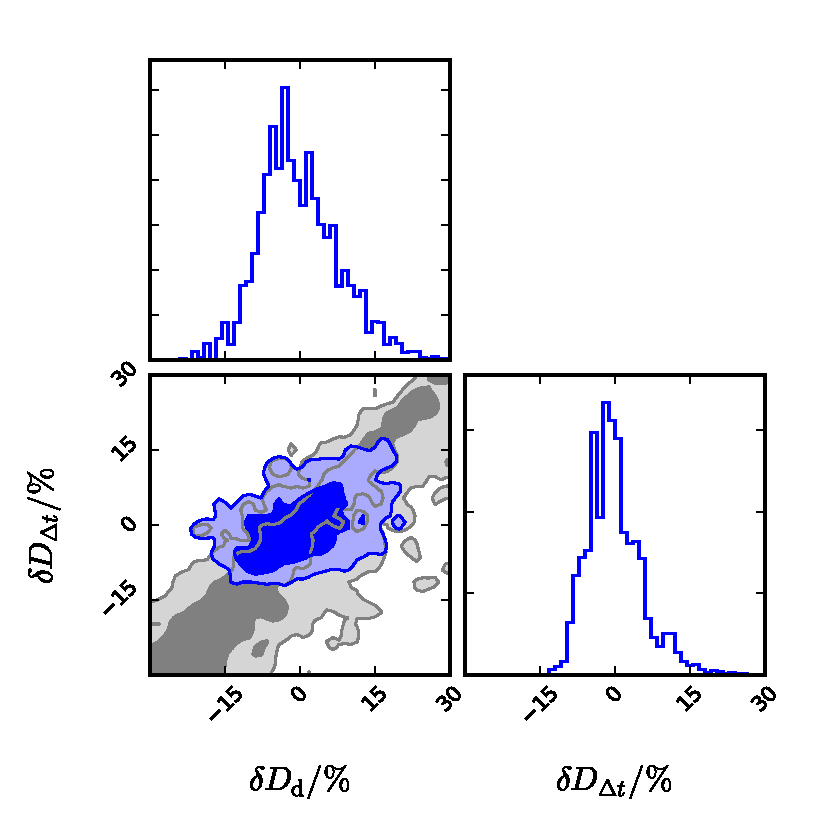
\includegraphics[width=\linewidth]{figures/B1608_DdtDa.pdf}
\end{minipage}
\caption{Cosmological information from angular diameter distances
as well as time delay distances. Left: Fisher matrix
forecasts for a future time delay lens sample where 5\% precision on
each distance is assumed: the combination of distances gives a
significantly more powerful constraint than the time delay distances
would alone \citep[reproduced from][]{JeeEtal2016}. ``$D_{\rm A}(EL)$'' is
the angular diameter distance to the lens from Earth. Right: marginalized
prior (gray) and posterior (blue) PDFs for the two
distances in the B1608$+$656 system, assuming uninformative priors for the
cosmological parameters of a flat $\Lambda$CDM model and offset and
rescaled to reveal the implied percentage precisions of 5.7\% and 8.1\%
in $\Ddt$ and $\Dd$ respectively (as shown by the vertical dashed lines
enclosing the 68\% credible region). }
\label{fig:DdDdt}
\end{figure*}
%%%%%%%%%%%%%%%%%%%%%%%%%%%%%%%%%


% {\bf TT: there is some repetition between the following paragraph and
% 6.3. Phil and Tommaso to decide how to resolve it. PJM: the simplest
% thing is simply to comment this out, and leave it for the roadmap. I
% think this makes sense: the whole roadmap section is about what it will
% take to reach the prescribed levels of precision and accuracy.}
%
%
% What will it take to reach the required level of distance precision in
% each of 100 lenses?  According to the data challenge summarized by
% \citet{LiaoEtal2015}, samples of over 100 lenses with
% precise time delays should be able to be constructed from analysis of
% the LSST light curves. The lens models for these systems should be
% able to be constrained to sufficient precision using high resolution
% imaging from next generation AO facilities, giant segmented mirror
% telescopes, JWST and even WFIRST \citep{Men++15}. High overall mass
% model precision, and the exploitation of the angular diameter distance
% dependence, will require high signal to noise ratio,
% spatially-resolved spectroscopy as well: integral field units on these
% same telescopes should be able to provide this. The contribution to
% the distance uncertainty from the line of sight was particularly high
% in the cases of B1608$+$656 and RXJ1131: in most other systems in a
% large sample the effects of the environment should be lesser, and they
% should (effectively) average down \citep{ColletEtal2013}.


% % % % % % % % % % % % % % % % % % % % % % % % % % % % % % % % % %

\subsection{Accuracy}
\label{ssec:accuracy}

While the precision available from Stage~III and Stage~IV samples makes
time delay lenses an interesting prospect for cosmology, they will,
like the other probes, be limited by systematic errors. As the
forecasts show, competitive contributions to joint dark energy
parameter inferences correspond to sub-percent precision in
characteristic distance, which implies that the residual systematic
(that is, post-combination error on the mean, sometimes referred to as
bias) error in distance needs to be well below 1\%. This residual
systematic may or not be present at this level in every lens system --
what matters is the bias in the overall measurement from the combined
sample. However, the term ``mean accuracy per lens'' is helpful, since
it reminds us that systematic errors can affect all members of a sample
in the same (or at least similar) way.  In
this section we revisit the primary sources of systematic error and
assess the prospects for this stringent requirement to be met.

\subsubsection{Time delay measurement}

\citet{LiaoEtal2015} showed that a
mean accuracy of 0.1\% per lens would already be achievable in
plausible samples of several hundred LSST lenses, were all images to
be taken in the same band.  While these results are encouraging,
questions about our ability to measure time delays from sparse,
multi-filter light curves extracted at scale from realistic images
remain \citep{TCM13}.  Time delay measurement accuracy from LSST
multi-filter light curve could be tested by a second challenge; the
success of the analyses is likely to hinge on the treatment of quasar
color variability \citep[see e.g.\ ][and references
therein]{Sch++12,SunEtal2014} and chromatic microlensing
\citep[see e.g.][and references therein]{HainlineEtal2013}.
Joint inference from whole samples is likely to
be important, in mitigating against both outliers and also imprecision
arising from inappropriate uniform priors on  population parameters.
Insights into AGN physics and the stellar composition  of lens galaxies
would be welcome by-products of such an analysis. An alternative approach
could be to continue to pursue single-filter monitoring, but at
increased efficiency. Experiments with higher cadence campaigns,
exploiting the short (sub-day) timescale variability of AGN are in
progress \citep[][F.~Courbin, priv.\ comm.]{BorosonEtal2016}.

It is worth noting that time delay {\it perturbations},  due to small
scale structure in lens plane or along line of sight, will likely not be
a significant  additional source of systematic error, since they
primarily cause additional scatter on hour-long timescales
\citep{K+M09}.


\subsubsection{Lens mass modeling}

\citet{S+S13} have pointed out the possibility of systematic errors at
the twenty percent level due to modeling assumptions (and their
interaction with the mass sheet degeneracy) when fitting lensing data
alone. \citet{Suy++14} fitted the same two models used by
\citet{S+S13}  to the current state of the art Einstein ring imaging and
lens galaxy velocity dispersion data, and found that present
measurements of stellar kinematics reduces the error by a factor of
10.  It is not clear how much of the residual 2\% uncertainty is
random, and how much residual bias there is: we do not yet know how
our mass modeling methods respond to the variety of lens mass
distributions we expect.

An important first step has been taken by \citet{XuEtal2016}, who
looked at the density profiles of a sample of mock galaxies from the
Illustris simulation, finding significant departures from simple power
law profiles. However, they note that at the mass scales typical of
galaxy scale lenses, where the total mass density profiles happen to
be well approximated by isothermal spheres
\citep{Koo++09,Aug++10}, the residual systematic uncertainty
in the Hubble constant could be restricted to a few percent.
Again, it remains to be verified how much of this averages out
given particular, large samples of systems.

As a result of these investigations, we know that 1) the dynamical
information is as important as the lensing data, 2) more complex
models than simple power law density profiles will likely be needed to
enable sub-percent accuracy to be reached, and 3) we now have
simulated galaxies that are {\it sufficiently realistic and suitably
complex} that we can carry out meaningful tests where the ground truth
is very different from our assumed analysis models. The acid test will
be whether we can recover the input cosmological parameters from
realistic simulated high resolution imaging and stellar spectroscopic
data made using numerical simulations that resolve massive
galaxies well \citep[e.g.,][]{Fia++16}.

As we look ahead to samples of dozens to hundreds of lenses in the
next decade, we can also consider the observational capabilities we
will have in that time period. Giant segmented mirror telescopes
(including the James Webb Space Telescope as well as planned 30m class
ground-based telescopes) will bring up to a factor of 10 increase in
angular resolution beyond what HST and today's 10-m class adaptive
optics-enabled telescopes can deliver, improving further the available
Einstein ring constraints. These facilities will be instrumented with
Integral Field Unit spectrographs, that will provide
spatially-resolved spectrocopy of the lens galaxy stellar populations.
It is yet to be seen how accurately lens mass distributions can be
modeled with such data: extending the realistic lens galaxy data
simulation work to include them would seem to be very important. The
``crash test'' of \citet{Bar++09a} was an excellent start in this
direction, probing as it did the performance of a fully self-consistent
lensing and dynamics modeling code on a numerically simulated lens
galaxy mock dataset.

The upcoming increase in available precision per lens will support
significantly more flexible mass models, as reviewed in
Section~\ref{ssec:lensmodel}.
%While early efforts in this
%direction employed regularized grids of pixels
%\citep{Koo05,SuyuEtal2009,V+K09a}, the most recent attempts model
%perturbations to simple density profiles with orthogonal basis sets
%\citep{BirrerEtal2015}.
The opportunity here is to find a flexible mass model whose parameters
can be taken to have been drawn from a relatively simple prior PDF,
which could be derived from either large samples of observed non-lens
galaxies, plausible hydrodynamic simulated galaxies, or both.


The mass sheet degeneracy, and indeed all model parameter degeneracies
are broken by incorporating more information, but this needs to be
done in such a way as to not introduce bias. Using flexible mass
models with reasonably broad but not uninformative priors is the first
step, but unless these priors are themselves movable, the introduced
bias might remain. The clear-cut solution is to learn the
hyper-parameters that govern the intrinsic distribution of mass model
parameters from the data as well. It is really the prior on these
``hyper-parameters'' that needs to come from simulations. An initial
attempts at this kind of ``hierarchical inference'' can be found in
the analysis of \citet{SonnenfeldEtal2015}, where the authors infer
the values of some 28 hyper-parameters assumed to govern the scaling
relations between massive galaxies, as well as the selection function
of the lens sample. As surveys yield larger and larger samples of
lenses, we can think of carrying out joint inferences with ensembles
of both time delay lenses, and also all other lenses, to bring in more
information about the density structure of somewhat self-similar
massive galaxies.

In addition to carrying out tests on simulated data, it is important
to continue empirical investigations of systematic errors. In addition
to the generally applicable strategy of comparing the cosmological
parameter estimates between individual systems or subsets of systems
to measure whether statistical uncertainties are under-estimated, we
must continue to look for other independent tests. An interesting
example is that of multiply imaged supernova Refsdal. Several teams
carried out lens models to predict in a truly blind fashion the
magnification, timing, and position of the next appearance of the
supernova \citep{Ogu15,S+J16,Jau++16,Tre++16,Kaw++16,Gri++16}. Even
though the deflector is a merging cluster, and thus dramatically more
challenging to model than the typical relaxed elliptical galaxies used
in time-delay cosmography, several teams managed to predict the event
\citep{Tre++16,Kel++16}  within the estimated uncertainties.  
It is particularly re-assuring that the code GLEE designed and used
extensively to model time delay cosmography
\citep{Suy++10,Suy++13,Suy++14} performed the best
\citep{Gri++16}. As the precision of time delay cosmography increases
with sample size it will be important to seize any new opportunity to
carry out additional blind tests, e.g. by predicting time delays of
lens quasars before measuring and by actively searching for multiply
imaged supernovae in galaxy-scale lenses \citep{O+M10}.


\subsubsection{Environment and line of sight characterization}

The current methodology (Section~\ref{ssec:los}) includes dependencies
on both cosmological simulations and reference imaging surveys. The
Stage~III and~IV wide field surveys will help with the latter,
providing much larger, more homogenous sets of control fields.
Systematic errors associated with calibrating against simulations is
the bigger problem, and both the number counts and 3D reconstruction
approaches that have been implemeted to date are affected.
\citet{CollettEtal2013} give some indication of the magnitude of the
issue, finding a bias of 3\% in the average inferred time delay distance
when assuming a stellar mass to halo mass relation that is incorrect
but still consistent with other observations. This reduces to 1-2\%
if the bright galaxies in the lens fields have spectroscopic redshifts,
suggesting that this kind of data will continue to be important.

The 3D reconstruction approach can, in principle, be made to be
independent from simulations \citep[indeed, this was a design feature
of][]{McCullyEtal2014}.  However, more  more information about mass in
the universe will be required.  Both \citet{McCullyEtal2014} and
\citet{CollettEtal2013} use halo models, with very simplistic treatments
of the mass outside of halos, and the voids between them. Both weak
shear data and clustering information could be used to improve the
accuracy of these  models; statistical halo models are already well
constrained by summary statistics from these probes
\citep[e.g.][]{CouponEtal2015},  and these results are already
potentially useful (although the scatter in the model's relations needs
will likely need to be taken into account).  Covariance with cosmic
shear, galaxy clustering, and the halo mass function may then  need to
be accounted for in any joint cosmological parameter inferences; this
may turn out to be negligible, but it needs to be quantified.  Some
mitigation of the environment and line of sight systematics could be
achieved by selecting low density lines of sight
\citep{CollettEtal2013}, but this selection would need to be done with
some care, propagating all the uncertainties.


Even when all the above systematics have been investigated and tested
for, others that are unforeseen may remain. Strategies for detecting
these ``unknown unknowns'' include jack-knife testing, which  will
become possible with larger samples. Other kinds of ``null tests'' may
also be possible when we are out of the small number stastistics regime:
research is needed on developing such tests. The ultimate test is
cosmological parameter consistency with other datasets, but for this
comparison be meaningful the analysis of each dataset must be done
blindly, to avoid unconscious experimenter bias and the resulting
groupthink towards (or away from) concordance
\citep[see e.g.][]{Con++06,Suy++13}. In principle all the
systematics tests  need to be done before unblinding; as a result, end
to end tests on highly realistic mock data will become ever more
important. The time delay challenge was carried out blind;
similarly-designed lens modeling and environment characterization
challenges are needed too. Success at blind cosmological parameter
recovery from realistic mock samples is the surest way to generate
confidence in a probe's accuracy.


% % % % % % % % % % % % % % % % % % % % % % % % % % % % % % % % % %

\subsection{Roadmap}
\label{ssec:roadmap}

We conclude the outlook section by proposing an ambitious, yet (in our
opinion) feasible roadmap for time delay cosmography in the next
decade. This roadmap aims to achieve $\sim0.5$ precision on time delay
distance\footnote{For simplicity, we refer to equivalent uncertainty
on an average time delay distance at the typical redshift of the
deflector and source. In practice of course, there will be a
distribution of redshifts and thus of invididual distances. As the
dependency of the time delay distance on cosmological parameters
changes slightly with redshift, the analysis of a real sample of
lenses will have the added benefit of breaking some of the
degeneracies and reducing the uncertainties more rapidly than if all
the systems were at the same redshift.} by 2027,
building on the tools and techniques demonstrated in
the past 15 years and exploiting the large scale surveys that are
currently under way or planned. It is based on a specific strategy,
consisting of constructing the most precise and accurate models of
each lens based on rich datasets for each system (alternative
strategies are discussed at the end of this section). Specifically,
for each system one needs the following:

\begin{enumerate}
\item Time delays precise to better than $3\%$;
\item High resolution imaging (resolution much better than the Einstein
radius) with point spread function known well enough to reconstruct the
differences in Fermat potential to better than $3\%$ precision;
\item Spectroscopic redshifts of the deflector and the source;
\item Stellar velocity dispersion of the deflector to better than 5\%
precision, possibly spatially resolved;
\item Imaging and spectroscopic data sufficient to characterize the
weak lensing effects due to structure along the line of sight to better than
$3\%$ precision.
\end{enumerate}

These targets can be met with present technology, as it has already
been demonstrated for a few systems \citep{Tew++13,Suy++13}, and the
observational requirements have been investigated for a variety of
telescopes and configurations
\citep{Gre++13,CollettEtal2013,Men++15,Lin15}.

%%%%%%%%%%%%%%%%%%%%%%%%%%%%%%%%%%%%%%
\begin{figure*}
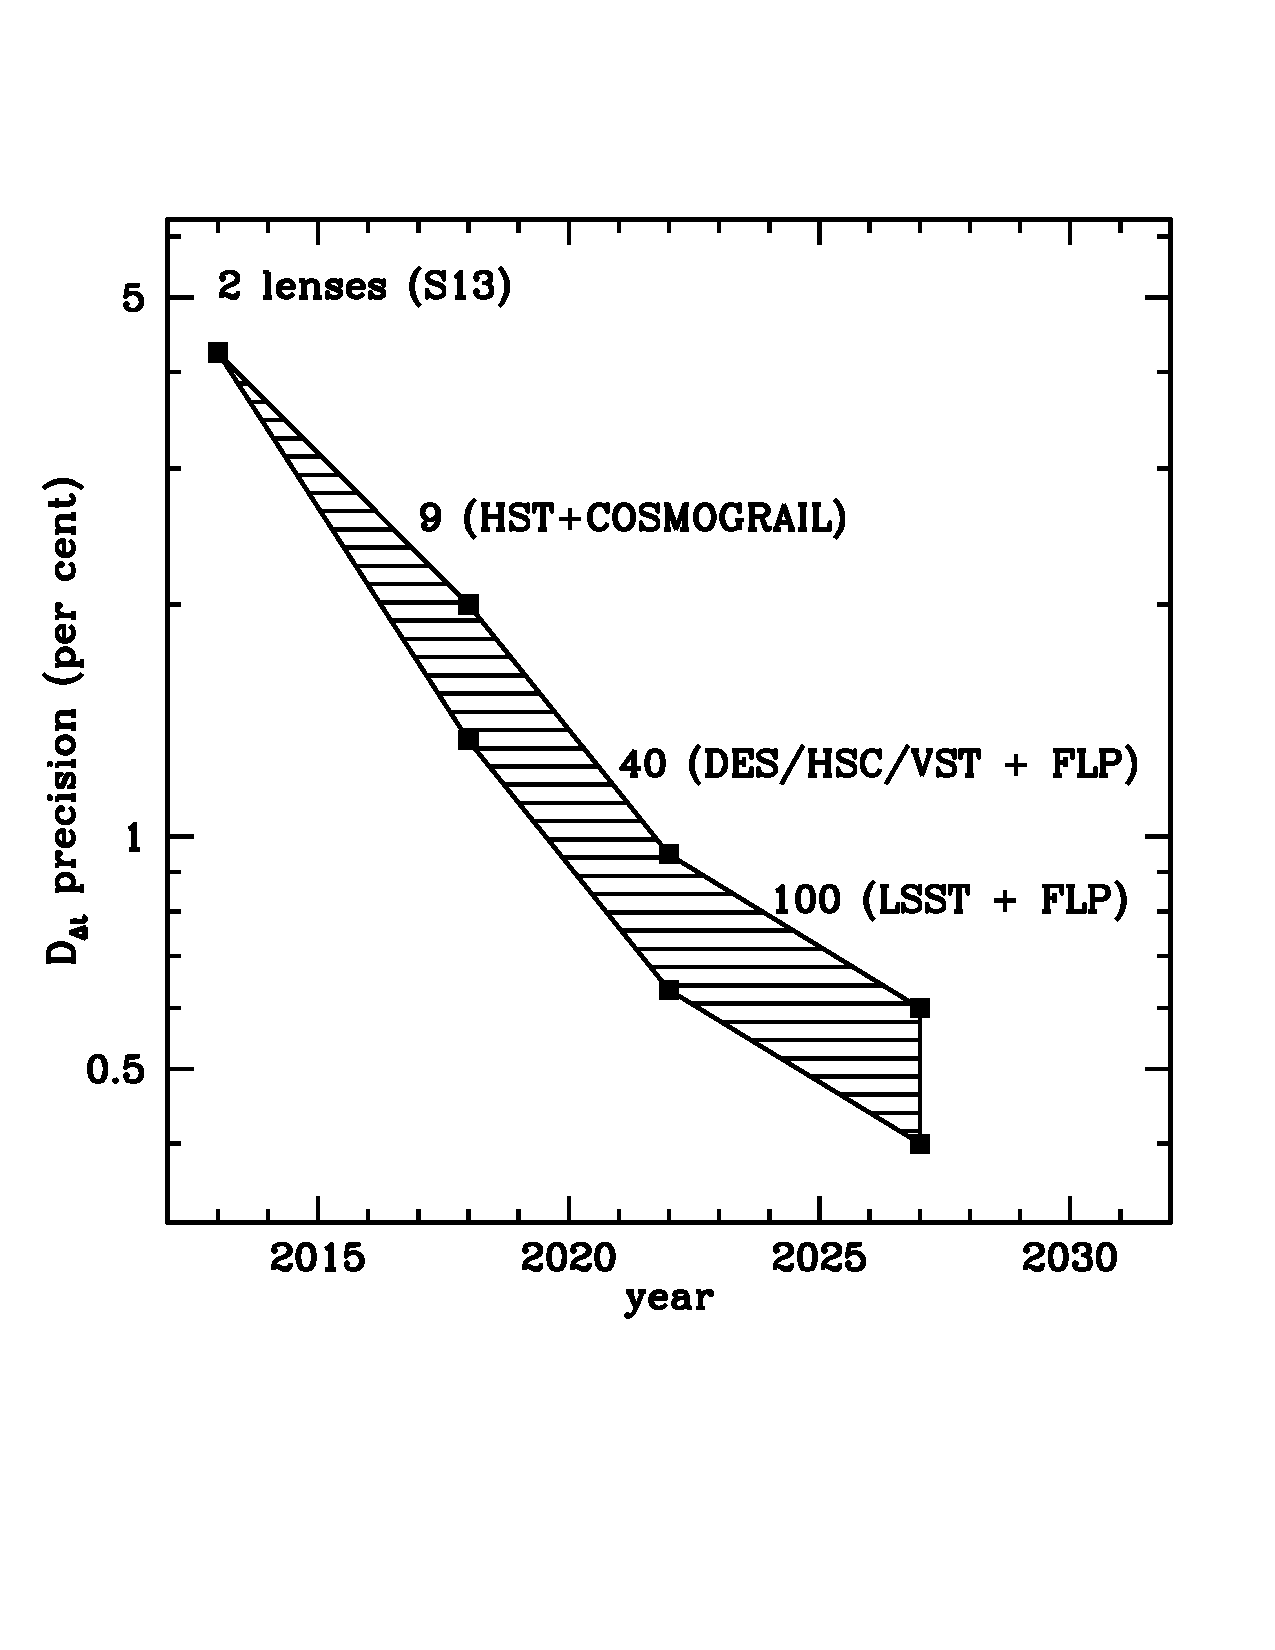
\includegraphics[width=0.98\textwidth]{figures/roadmap.pdf}
\caption{Roadmap for time delay cosmography. The shaded region
represents the estimated range of uncertainty attainable on the
effective (ensemble) time delay distance $\Ddt$ as a
function of time, over the next ten years.}
\label{fig:roadmap}
\end{figure*}
%%%%%%%%%%%%%%%%%%%%%%%%%%%%%%%%%%%%%%

The proposed roadmap is summarized in Figure~\ref{fig:roadmap}. The
shaded region represents an estimate of the ensemble precision attainable on
$\Ddt$ (which \citet{C+M09b} call $\mathcal{\tau}_{\rm C}$),
ranging from the most conservative to the most favorable
scenario. The most conservative case assumes only a central velocity
dispersion measurement for each system, while the most favorable
scenario involves spatially resolved stellar velocity dispersions,
obtained either from space or from the ground assisted by adaptive optics
(Agnello et al. 2016, in prep). We neglect the additional independent
information that in principle can be obtained via the angular
diameter distance dependence \citep{JeeEtal2016}.  As
discussed in Section~\ref{ssec:precision}, this additional piece of
information would in principle improve the constraints on cosmological
parameters from time delay lenses, so this envelope should be regarded
as a conservative estimate.

The roadmap is divided into steps, whose timing is dictated by
available observational facilities.
The first step in the roadmap is the analysis
of two systems that was published in 2013, and was based on COSMOGRAIL time
delays, HST imaging, Keck spectroscopy, and other ancillary data from
a variety of sources.

The second step consists of the full analysis of
nine lens systems for which time delays have been measured by the
COSMOGRAIL team, and for which HST imaging is being completed this
year. Completing the second step by the launch of the James Webb Space
Telescope at the end of 2018,
and in doing so delivering $\sim2\%$ distance precision,
would be ideal, so as to provide a useful
comparison for expected improvements in local distance ladder
measurements.

The third step will require the discovery of new lenses, in addition
to the usual follow-up effort. Systematic searches are currently under
way based on large scale surveys such as the Dark Energy survey
\citep{Agn++15,Mor++16}, and should
discover hundreds of new lensed quasar systems by the
end of the decade \citep{O+M10}.
Focused follow-up of a carefully selected sample of
systems should be sufficient to reach the goal for step 3, that is,
$\sim1\%$ distance precision from 40
lenses in 5 years (i.e. by 2022). The selected sample should
consist of as many quads as possible, since they contain more
cosmological information and favor systems with time delays in the
range 50-150 days, such that they are measurable at the
$<3\%$ level in one observing
season with daily cadence. The observational bottle necks are likely
going to be first the time delay measurements, which will require
dedicated monitoring on 1--4m class telescopes, and high resolution
imaging \citep{Tre++13}.

Scaling up to the fourth step will require a change of strategy, in
order to cope with the intrinsically fainter targets and larger sample
size. One natural strategy will consist of using time delays measured
from LSST light curves \citep{LiaoEtal2015}, perhaps supplemented in
part from 1--4m telescopes in order to increase the cadence, or potentially
from a dedicated lens monitoring satellite
\citep{Mou++08}. Unfortunately, LSST imaging will be insufficient for
detailed modeling, and higher resolution imaging will be required
\citep{Men++15}.
Planned surveys like Euclid and WFIRST will be excellent at
discovering new lenses, but probably will have insufficient depth and
resolution except for the brightest systems. Therefore targeted
follow-up will be required, achievable either with JWST from space, or
with improved adaptive optics systems on 8--10m class ground-based
telescopes. Integral field spectrographs on giant segmented mirror
telescopes will be the ideal complement to LSST, by providing the
necessary high resolution imaging and spetroscopy with relatively
short exposure times
\citep[e.g.][]{Ski++15}.
This fourth step
aims to reach $\sim0.5\%$ precision, through follow-up of systems discovered
and monitored in the first five years of the LSST survey.

Converting the uncertainty
in time delay distance $\Ddt$ to cosmological parameters requires
specific assumptions about the cosmological model and priors from
independent measurements. For step 1, the equivalent precision on H$_0$
using WMAP7 prior in one parameter extensions of $\Lambda$CDM is 4-5\%.
The forecast for step 2 with WMAP9 and Planck priors is shown in
Figure~\ref{fig:roadmap-step2}. For steps 3 and 4, the equivalent
precision on H$_0$ is in the range 1.1-1.3\% and 0.8\%-1.0\%
respectively, assuming ``Planck + Stage II'' priors \citep{C+M09b}.


%%%%%%%%%%%%%%%%%%%%%%%%%%%%%%%%%%%%%%
\begin{figure*}
\begin{center}
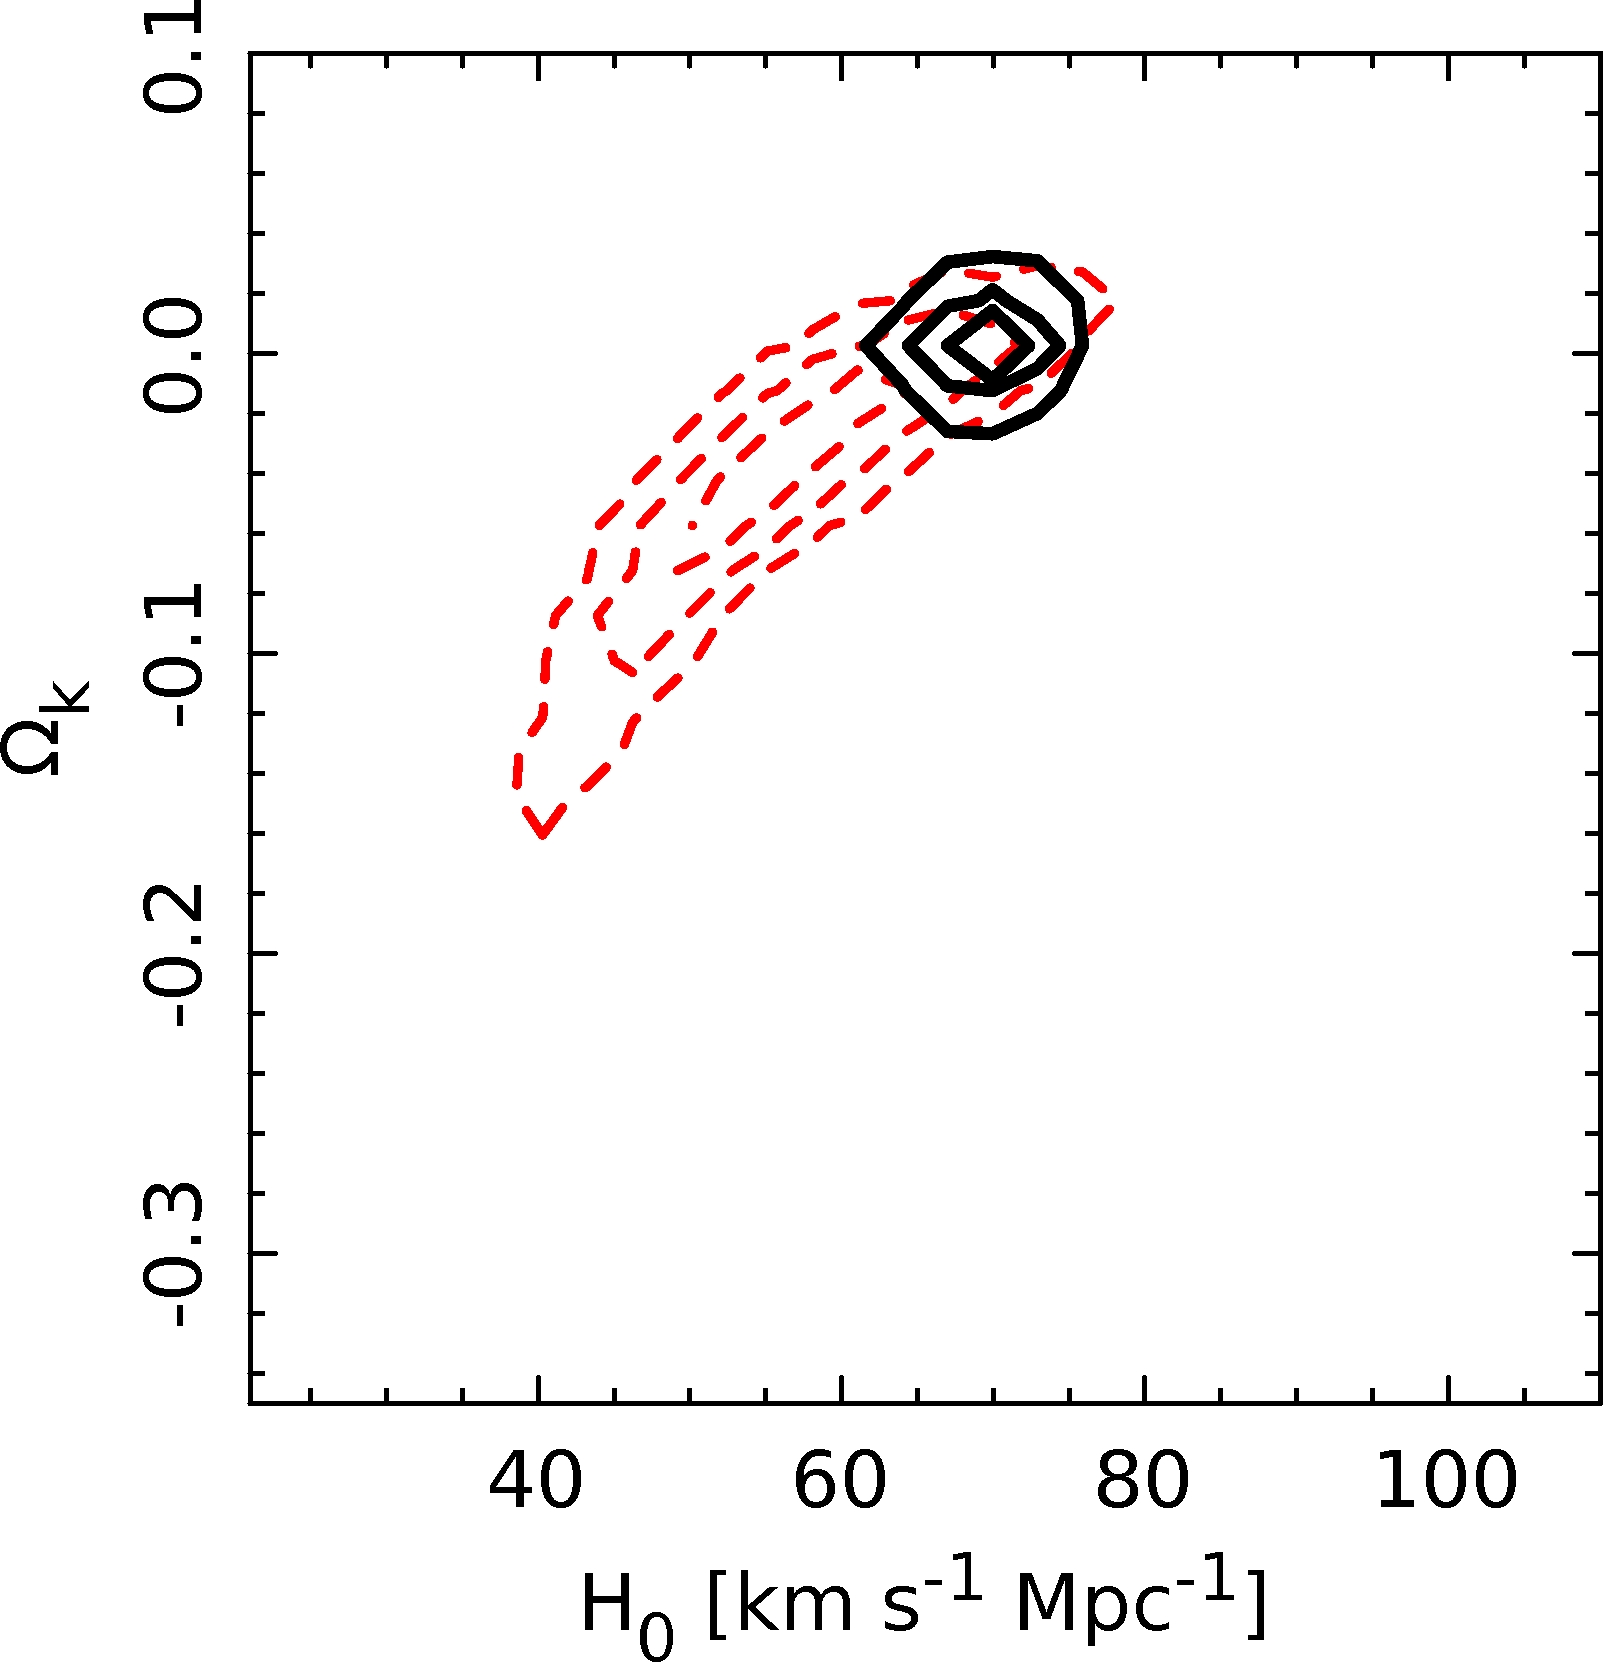
\includegraphics[height=5.5cm,clip]{figures/planck_olcdm_c22lenses_stats.jpg}
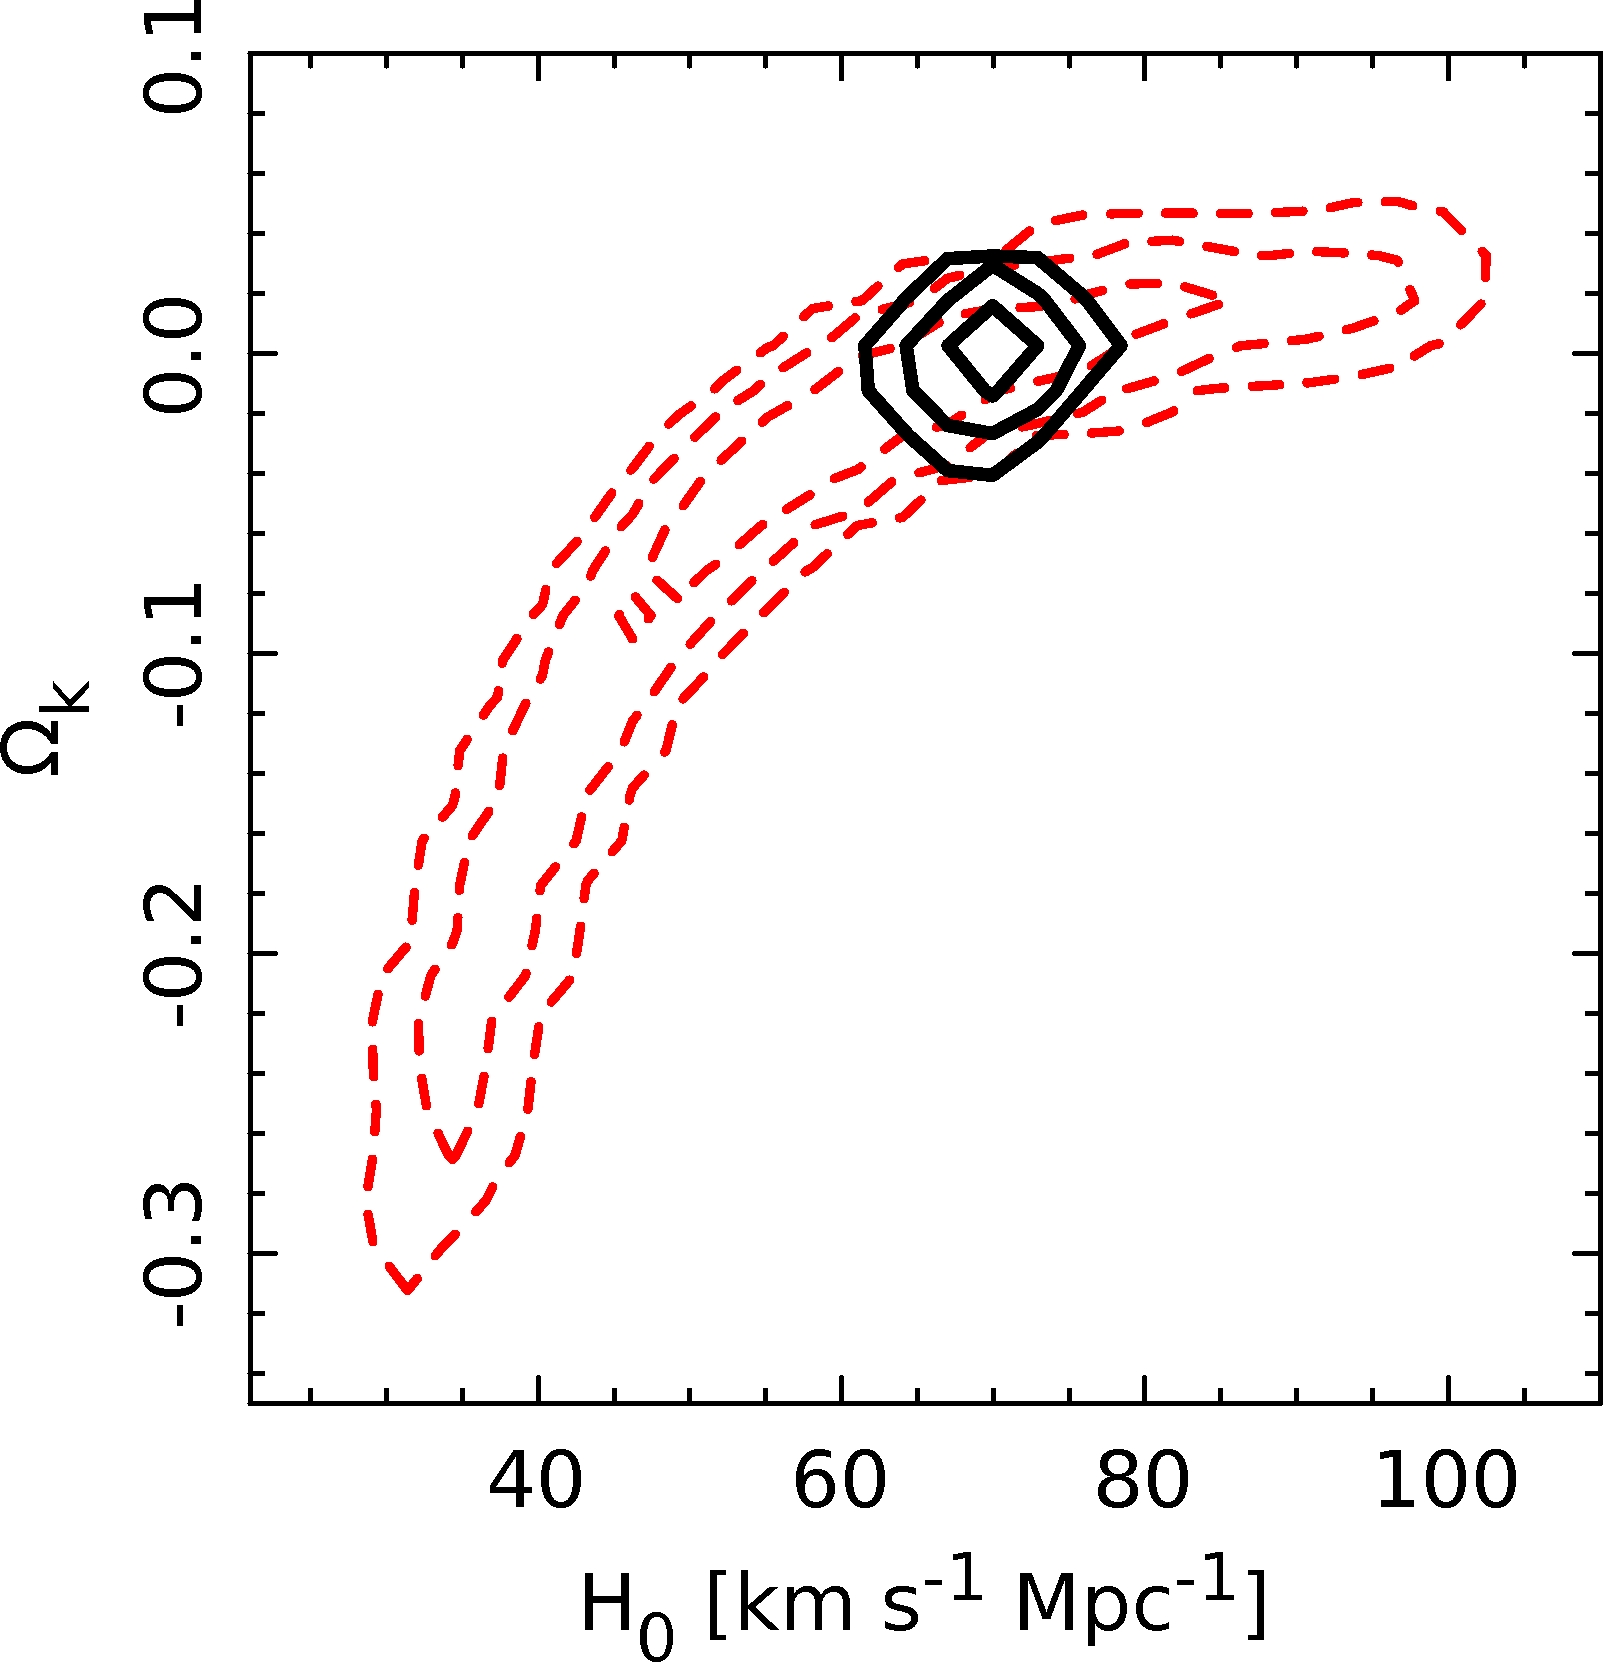
\includegraphics[height=5.5cm,clip]{figures/wmap9_olcdm_c22lenses_stats.jpg}
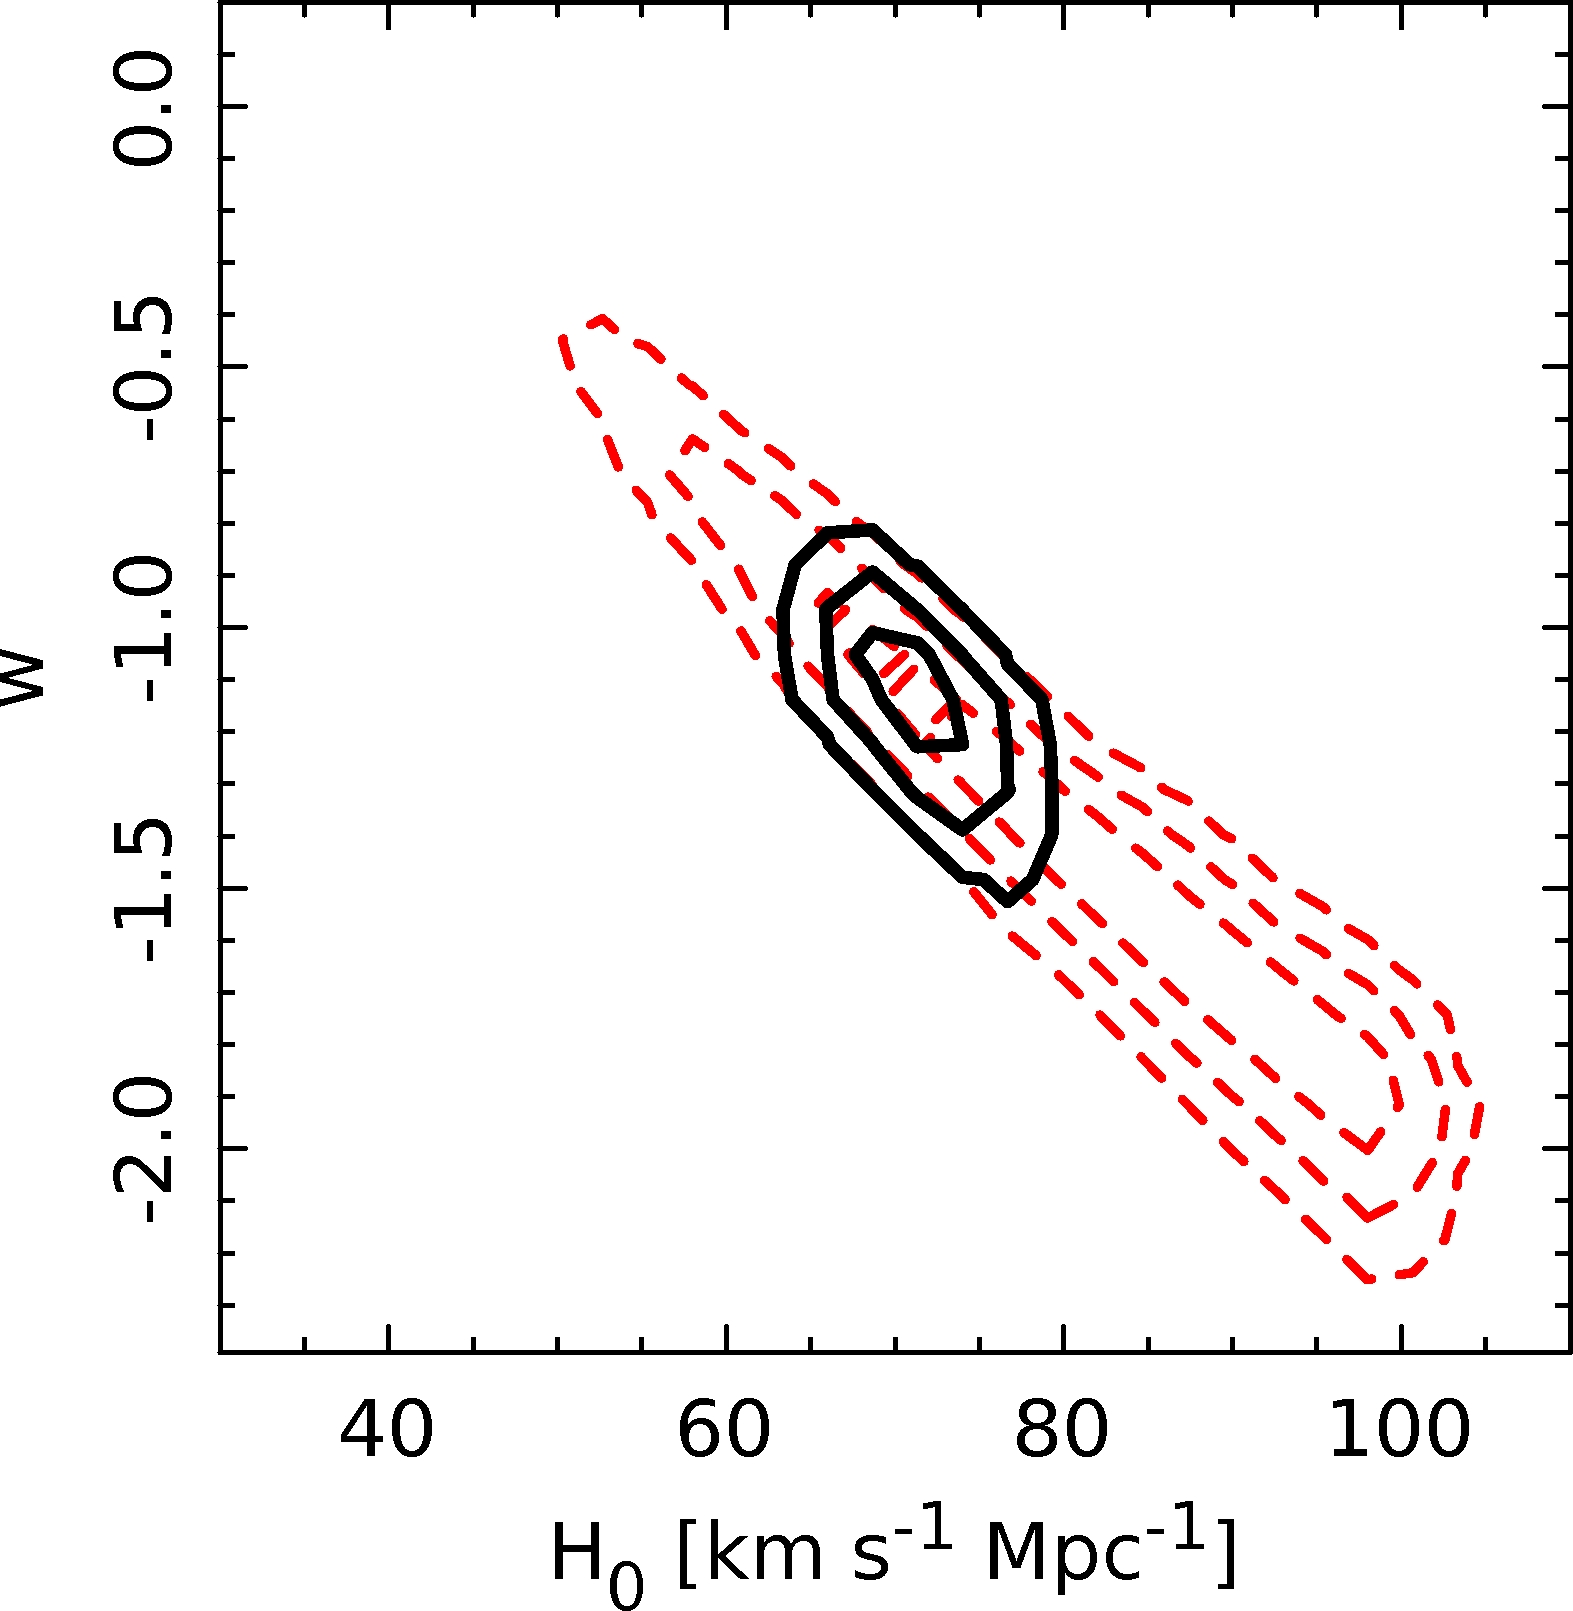
\includegraphics[height=5.5cm,clip]{figures/planck_wcdm_c22lenses_stats.jpg}
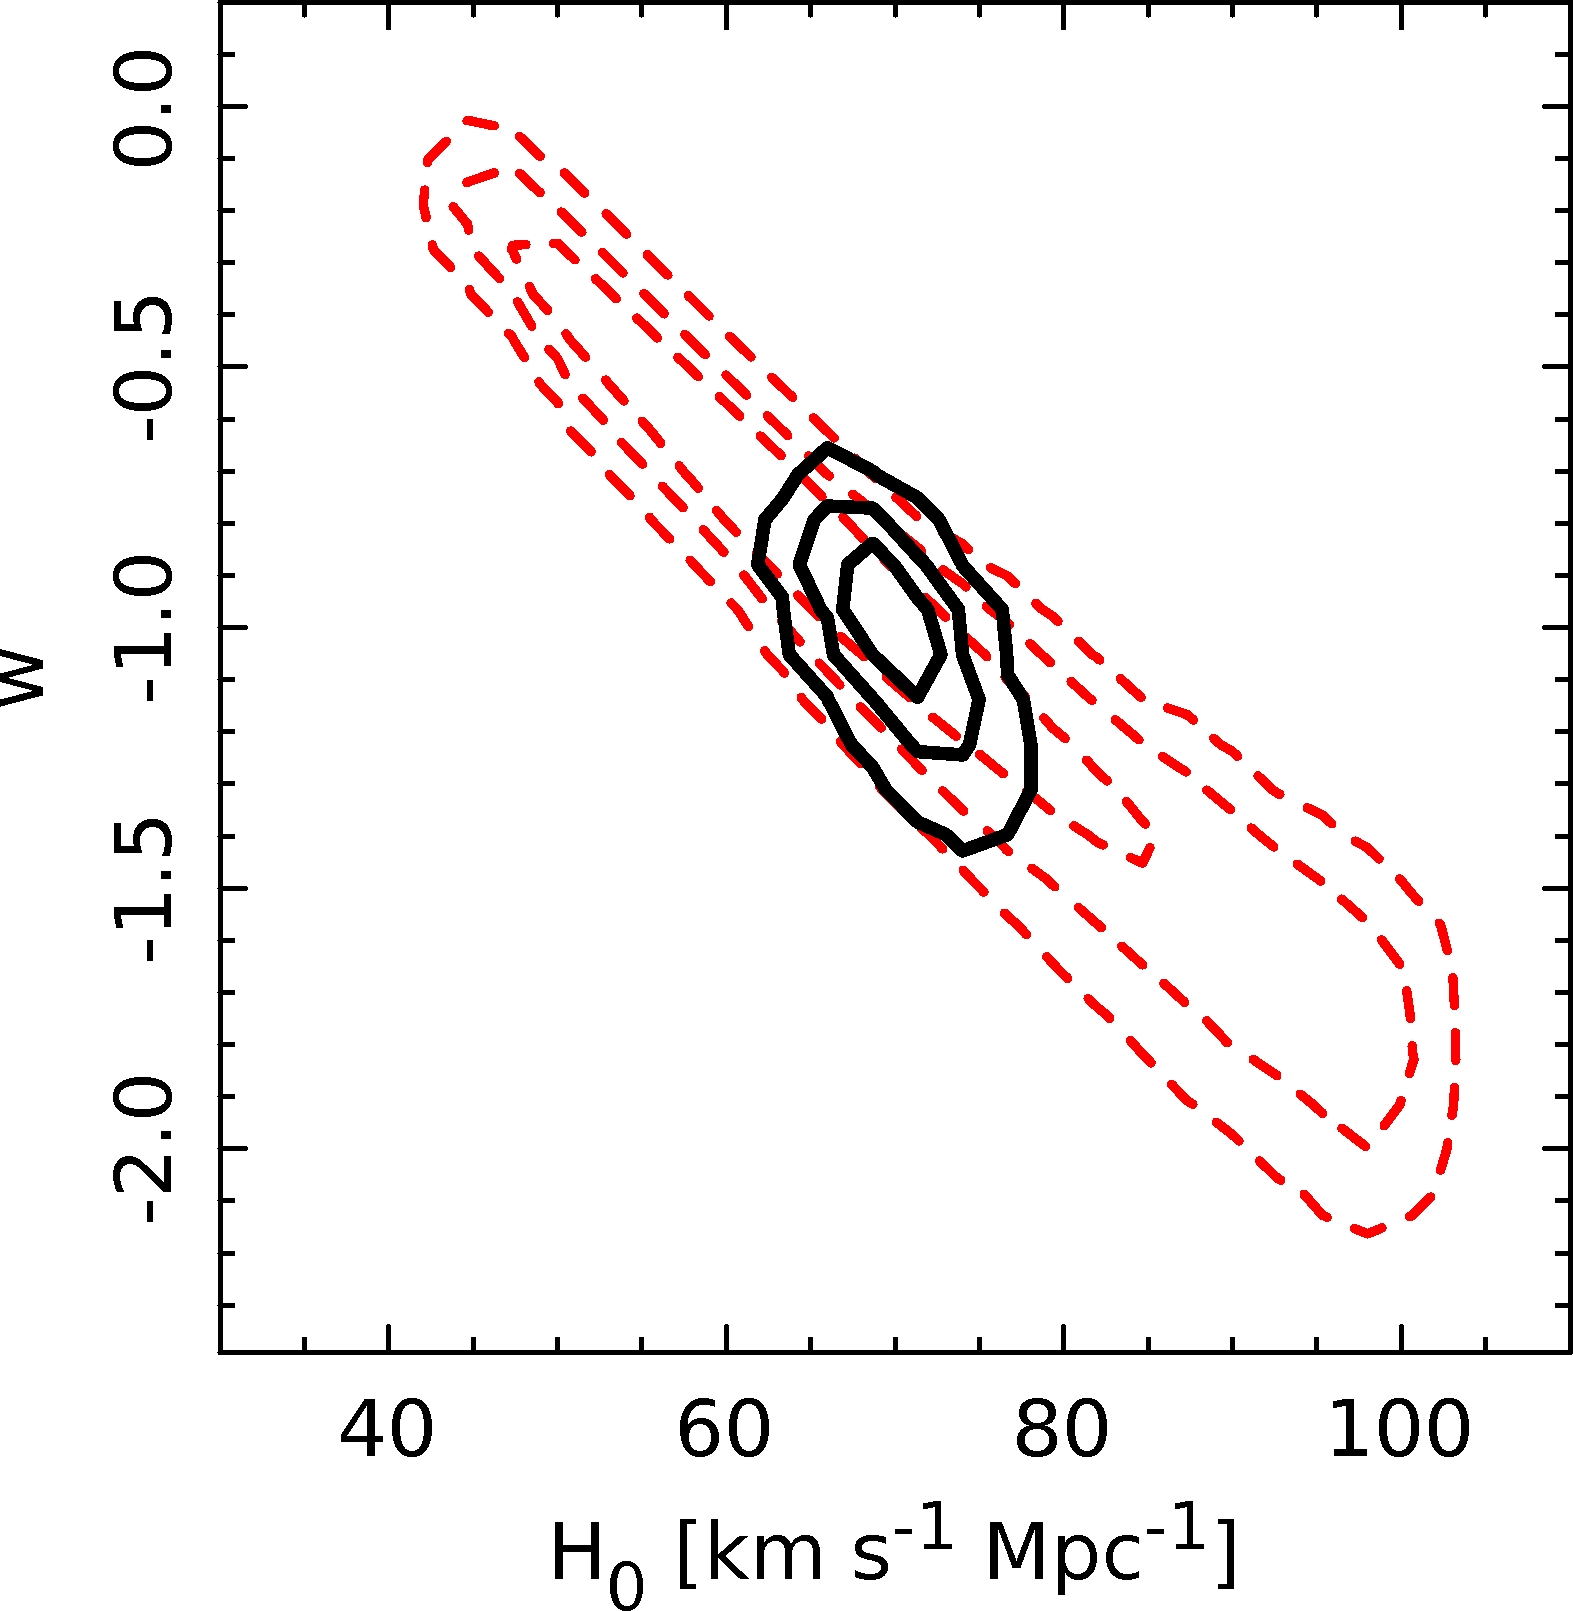
\includegraphics[height=5.5cm,clip]{figures/wmap9_wcdm_c22lenses_stats.jpg}
\end{center}
\caption{Cosmological forecast (black solid lines, represent the 68\%,
95\%, and 99\% posterior probability contours) for step 2 in the roadmap
(see Figure~\ref{fig:roadmap} and Section~\ref{ssec:roadmap} for
details), assuming one parameter extensions of flat $\Lambda$CDM, and
Planck (left column) and WMAP9 (right column) priors (red dashed lines).
Figure courtesy of S.H.~Suyu.}
\label{fig:roadmap-step2}
\end{figure*}
%%%%%%%%%%%%%%%%%%%%%%%%%%%%%%%%%%%%%%

In addition to the observational challenges, the main challenge in
pursuing this roadmap is likely to be the analysis cost. Lens modeling
is at present fairly labor intensive, requiring several months of work
per system by an expert modeler. This high labor cost is chiefly due
to code development. Up to now, the analysis of each single lens has
required the development and testing of new features (e.g. multi-plane
lensing, point spread function reconstruction). In order to analyze
the future large samples, the analysis codes will have to transition
from development to production, reducing substantially the
investigator time per system. Distributing the work among a large team
of modelers will likely be necessary to speed things up and keep
modeling uncertainties in check.

Naturally, this proposed roadmap is not the only possible way
forward. As discussed earlier in this section, several authors have
proposed the analysis of larger samples of lenses, each with fewer
ancillary data and thus lower precision per system. Alternatively, one
could imagine a hybrid strategy in which a subset of the lenses are
analyzed in great detail with lots of ancillary data, and the lessons
learned from that subset are propagated to a large sample through
judicious use of priors.
